
%\documentclass[manuscript,endfloat]{geophysics}
\documentclass[revised,endfloat]{geophysics}
%\documentclass[twocolumn,endfloat]{geophysics}

\usepackage{xy}
\usepackage{natbib}
\usepackage{graphicx}
\usepackage{url}
\usepackage{rotating}
\usepackage{lscape}
\usepackage{color}
\usepackage{rotating}
\usepackage{amsmath}
\usepackage{mathrsfs}
\usepackage{amssymb}      
\usepackage{algpseudocode}
\usepackage{booktabs}
 \usepackage{tikz}
 \usetikzlibrary{matrix}
 \DeclareMathAlphabet\mathbfcal{OMS}{cmsy}{b}{n}
 
\usepackage[ruled,linesnumbered]{algorithm2e}
\SetKwProg{Fn}{Function}{}{}

\usepackage{mathtools}
\DeclarePairedDelimiter\ceil{\lceil}{\rceil}
\DeclarePairedDelimiter\floor{\lfloor}{\rfloor}

\setlength\parindent{0pt}

\setlength\heavyrulewidth{0.25ex}

\DeclareGraphicsExtensions{.pdf}
\DeclareMathAlphabet\mathbfcal{OMS}{cmsy}{b}{n}
\DeclareMathOperator*{\argmin}{arg\,min}

\begin{document}

\title{Structured matrix}
\renewcommand{\thefootnote}{\fnsymbol{footnote}}

\address{
\footnotemark[1]Department of Physics,\\
University of Alberta, \\
Edmonton, Alberta, Canada. \\}

\author{Wenlei Gao\footnotemark[1]} 

\maketitle

%%%%%%%%%%%%%%%%%%%%%%%%%%%%%%%%%%%%%%%%%%%%%%%%%%%%%%%%%%%%%%%%%%%%%%%%%%%%%%
% ABSTRACT                                                                   %
%%%%%%%%%%%%%%%%%%%%%%%%%%%%%%%%%%%%%%%%%%%%%%%%%%%%%%%%%%%%%%%%%%%%%%%%%%%%%%

\begin{abstract}
The documentation for fast MSSA and relationship between multi-dimensional convolution and structured matrix, such as Circulant, Toeplitz and Hankel matrix.
\end{abstract}


%%%%%%%%%%%%%%%%%%%%%%%%%%%%%%%%%%%%%%%%%%%%%%%%%%%%%%%%%%%%%%%%%%%%%%%%%%%%%%
\section{Introduction}
\citep{korobeynikov2009} proposed the computation and memory efficient method for MSSA.
                                                                 
%%%%%%%%%%%%%%%%%%%%%%%%%%%%%%%%%%%%%%%%%%%%%%%%%%%%%%%%%%%%%%%%%%%%%%%%%%%%%%
\section{Method}
We start from the definition of discrete fourier transform.

\subsection{Discrete Fourier transform (DFT)}
For a vector ${\bf s}$ length of $N$, the discrete Fourier transform is  defined as
\begin{equation}
\tilde{s}_k  = \sum_{l=0}^{N-1} e^{-i 2 \pi k l / N} s_l \,,
\label{eq1}
\end{equation}
where the index $k = 0, 1, 2, \cdots, N-1$. Suppose the vector ${\bf s}$ represent a time series length of $N$ with time sampling interval is $\Delta t$. So the frequency sampling interval $\Delta f$ can be computed as 
\begin{equation}
\Delta f  = 1/ \Delta t / N = \frac{1}{N \Delta t}
\label{eq2}
\end{equation}
The Fourier transform for this time series in continueous case can be expressed as
\begin{equation}
\tilde{s}(f)  = \int e^{-i 2 \pi f t} s(t) dt 
\label{eq3}
\end{equation}
In discrete case and assume the frequency $f$ can be expressed as $f = k \Delta f$ and using the expression in equation \ref{eq2}
\begin{equation}
\begin{split}
\tilde{s}_{k \Delta f}  &= \sum_{l=0}^{N-1} e^{-i 2 \pi \, k \Delta f \,  l \Delta t} s_{l \Delta t}  \\
\tilde{s}_{k \Delta f}  &= \sum_{l=0}^{N-1} e^{-i 2 \pi \, k \frac{1}{N \Delta t} \,  l \Delta t} s_{l \Delta t} \\
\tilde{s}_{k}  &= \sum_{l=0}^{N-1} e^{-i 2 \pi \, k l / N} s_l \,.
\end{split}
\label{eq4}
\end{equation}
The the last equation is exactly same as the equation \ref{eq1}. Through this derivation, we can understand the physical meaning of the Fourier coefficients obtained via discrete Fourier transform. Note that the first coefficient corresponding to $0$ frequency and so as to the time series. The first element of ${\bf s}$ is the sample at $0$ time. 

The above operation can be expressed into the matrix-vector form. To simplify the definition of Fourier transform matrix, we define a variable $z = e^{-i \pi  / N}$, so the Fourier transform matrix, which is a $N$-by-$N$ square matrix and the element $F_{kl} = z^{kl}$. It can be expanded as
\begin{equation}
{\bf F}_N = \begin{bmatrix}
1 & 1 & \cdots & 1 \\
1 & z & \cdots & z^{N-1} \\
1 & z^2 & \cdots & z^{2(N-1)} \\
\vdots & \vdots & \ddots & \vdots \\
1 & z^{N-1} & \cdots & z^{(N-1)(N-1)} \\
\end{bmatrix}
\label{eq5}
\end{equation}
As ${\bf F}_N$ is a orthogonal (but not orthonormal) matrix, we can be easily get the its inverse matrix
\begin{equation}
{\bf F}_N^{-1} = \frac{1}{N} {\bf F}_N^H = \frac{1}{N} {\bf F}_N^{\ast} \,
\label{eq6}
\end{equation}
where the super-script $^H$ represent complex conjugate transpose and $\ast$ indicate conjugate transpose. As the matrix ${\bf F}_N$ is a symmetrical matrix, that's why we can get equation \ref{eq6}.

\subsection{Properties of Fourier transform}

In this section, we review the properties of discrete Fourier transform ({\bf DFT}), most of the properties are derived in continuous domain as it is much easier for the derivation, but the discrete version are verified by $Julia$ code.

We define the Fourier transform as
\begin{equation}
X(\omega) = \int_{-\infty}^{\infty} x(t) e^{-i\omega t} dt
\end{equation}
where $\omega$ is radian frequency and $t$ is time. The above operation can be simplified as 
\begin{equation}
{\mathbfcal F}[x(t)] \rightarrow X(\omega)
\end{equation}

\subsubsection{1. time shift}
\begin{equation}
{\mathbfcal F}[x(t-t_0)] = X(\omega)e^{i \omega t_0}
\end{equation}

{\bf Proof}:
$$
{\mathbfcal F}[x(t-t_0)]  = \int_{-\infty}^{\infty} x(t - t_0) e^{-i\omega t} dt  
$$
we set $t^{\prime} = t - t_0$ and exchange the variables, we can get
$$
{\mathbfcal F}[x(t-t_0)]  = \int_{-\infty}^{\infty} x(t^{\prime}) e^{-i\omega (t^{\prime} + t_0)} d t^{\prime}  $$
$$
{\mathbfcal F}[x(t-t_0)] = e^{-i \omega t_0} \int_{-\infty}^{\infty} x(t^{\prime}) e^{-i\omega t^{\prime}} d t^{\prime} = X(\omega) e^{-i \omega t_0}
$$

\subsubsection{2. frequency modulation}
\begin{equation}
{\mathbfcal F}[x(t)e^{i \omega_0 t}] = X(\omega-\omega_0)
\end{equation}
{\bf Proof}:
$$
{\mathbfcal F}[x(t)e^{i \omega_0 t}]  = \int_{-\infty}^{\infty} x(t)e^{i \omega_0 t} e^{-i\omega t} dt  \\
=  \int_{-\infty}^{\infty} x(t) e^{-i (\omega-\omega_0) t} dt  =  X(\omega-\omega_0)
$$
\textcolor{red}{Note: this is the property we forget very often.}

\subsubsection{3. time reversal}
\begin{equation}
{\mathbfcal F}[x(-t)] = X(-\omega)
\end{equation}
{\bf Proof}:
$$ {\mathbfcal F}[x(-t)]  = \int_{-\infty}^{\infty} x(-t)e^{-i \omega t} dt  $$
Set $t^{\prime} = -t$ and change the variables we can get
$$ {\mathbfcal F}[x(-t)]  = \int_{\infty}^{-\infty} x(t^{\prime}) e^{-i \omega (-t^{\prime})} d (-t^{\prime}) \\
= \int_{-\infty}^{\infty} x(t^{\prime}) e^{-i (-\omega) t^{\prime}} d t^{\prime} \\
= X(-\omega)$$
Based on this property, we can get two extensions, if the time function is and even function, that is
$$x(t) = x(-t) \rightarrow X(\omega) = X(-\omega)$$
if the time function is odd function, the Fourier transform of this function is also an odd function
$$x(t) = -x(-t) \rightarrow X(\omega) = - X(-\omega)$$

\subsubsection{4. time and frequency stretching}
\begin{equation}
{\mathbfcal F}[x(at)] = \frac{1}{a}X(\frac{\omega}{a})
\end{equation}
where $a$ is positive number

{\bf Proof}:
$$ {\mathbfcal F}[x(at)]  = \int_{-\infty}^{\infty} x(at)e^{-i \omega t} dt  $$
Set $t^{\prime} = a t$, By change the variable, we can get
$$ {\mathbfcal F}[x(at)]  = \int_{-\infty}^{\infty} x(t^{\prime})e^{-i \omega \frac{t^{\prime}}{a}} d\frac{t^{\prime}}{a} = \frac{1}{a}  \int_{-\infty}^{\infty} x(t^{\prime}) e^{-i \frac{\omega}{a} t^{\prime}} d t^{\prime} = \frac{1}{a}X{(\frac{w}{a})} $$
\textcolor{red}{Stretching in one domain means squeezing in another domain and vis versa.}

\subsubsection{5. Complex conjugate}
\begin{equation}
{\mathbfcal F}[x^*(t)] = X^*(- \omega)
\end{equation}
where the super-script $^*$ represent complex conjugate.

{\bf Proof}:
$$\int_{-\infty}^{\infty}  x^*(t) e^{-i \omega t} dt = \int_{-\infty}^{\infty} \left( x(t) e^{i \omega t}\right)^* dt = \int_{-\infty}^{\infty} \left(x(t) e^{-i (-\omega) t}\right)^* dt = \left( \int_{-\infty}^{\infty} x(t) e^{-i (-\omega) t} dt\right)^* = X^*(-\omega)  $$


\subsection{Circulant matrix}
An $9 \times 9$ circulant matrix is defined as
\begin{equation}
{\bf C} = 
\begin{bmatrix}
c_1 & c_9 & c_8 & c_7 & c_6 & c_5 &  c_4 & c_3 & c_2 \\ 
c_2 & c_1 & c_9 & c_8 & c_7 & c_6 &  c_5 & c_4 & c_3 \\ 
c_3 & c_2 & c_1 & c_9 & c_8 & c_7 &  c_6 & c_5 & c_4 \\ 
c_4 & c_3 & c_2 & c_1 & c_9 & c_8 &  c_7 & c_6 & c_5 \\ 
c_5 & c_4 & c_3 & c_2 & c_1 & c_9 &  c_8 & c_7 & c_6 \\ 
c_6 & c_5 & c_4 & c_3 & c_2 & c_1 &  c_9 & c_8 & c_7 \\ 
c_7 & c_6 & c_5 & c_4 & c_3 & c_2 &  c_1 & c_9 & c_8 \\ 
c_8 & c_7 & c_6 & c_5 & c_4 & c_3 &  c_2 & c_1 & c_9 \\ 
c_9 & c_8 & c_7 & c_6 & c_5 & c_4 &  c_3 & c_2 & c_1 \\ 
\end{bmatrix}
\end{equation} 
A circulant matrix is fully specified by its first column ${\bf c} = \begin{bmatrix}
c_1 & c_2 &  c_3 &  c_4 &  c_5 &  c_6 &  c_7 &  c_8 &  c_9  \end{bmatrix}^T$, we know that the product between circulant matrix and a vector ${\bf v}$ length of $N$ is equivalent to the circular convolution between vector ${\bf c}$ and ${\bf v}$, and the circular convolution can be computed efficiently via Fast Fourier transform (FFT). So we have
\begin{equation}
{\bf Cv} = {\bf F}_N^{-1} \left(  {\bf F}_N {\bf c} \circ {\bf F}_N {\bf v} \right)  =  {\bf F}_N^{-1} \left(  diag({\bf F}_N {\bf c}) \cdot {\bf F}_N {\bf v} \right) \,,
\end{equation}
where the symbol $\circ$ and $diag$ represents Hardmard (element-wise) multiplication and building diagonal matrix from a vector.

\subsection{Toeplitz matrix}
Toeplitz matrix is associated with linear convolution, suppose we have two vectors ${\bf s} = \begin{bmatrix}  s_1 & s_2 & s_3 & s_4 & s_5  \end{bmatrix}^T$ and ${\bf f} =  \begin{bmatrix}  f_1 & f_2 & f_3 & f_4 & f_5  \end{bmatrix}^T$,  the linear convolution of these two vectors is vector ${\bf r}$ length of $9$. We can represent the convolution into matrix-vector form as
\begin{equation}
{\bf r} = {\bf  h} \ast {\bf f} = \begin{bmatrix}
r_1 \\
r_2 \\
r_3 \\
r_4 \\
r_5 \\
r_6 \\
r_7 \\
r_8 \\
r_9 \\
\end{bmatrix}
= \begin{bmatrix}
s_1    & \quad & \quad & \quad & \quad  \\ 
s_2    & s_1    & \quad & \quad & \quad  \\ 
s_3    & s_2    & s_1 & \quad & \quad \\ 
s_4    & s_3 & s_2 & s_1 & \quad  \\ 
s_5    & s_4 & s_3 & s_2 & s_1  \\ 
\quad & s_5 & s_4 & s_3 & s_2 \\ 
\quad & \quad & s_5 & s_4 & s_3  \\ 
\quad & \quad & \quad & s_5 & s_4 \\ 
\quad & \quad & \quad & \quad & s_5  \\ 
\end{bmatrix}
\begin{bmatrix}
f_1 \\
f_2 \\
f_3 \\
f_4 \\
f_5 \\
\end{bmatrix}
\end{equation}
The efficient linear convolution usually padding $0$ to vectors make their length equal to $9$, after padding zeros, we get new vector $\hat{\bf s} = \begin{bmatrix}  s_1 & s_2 & s_3 & s_4 & s_5 & 0 & 0 & 0 & 0 \end{bmatrix}$ and  $\hat{\bf f} = \begin{bmatrix}  f_1 & f_2 & f_3 & f_4 & f_5 & 0 & 0 & 0 & 0 \end{bmatrix} $, the circular convolution between $\hat{\bf s}$ and $\hat{\bf f}$ can be expressed as
\begin{equation}
\hat{\bf r} = \hat{\bf s} \circledast \hat{\bf f} = \begin{bmatrix}
s_1 & 0     & 0     & 0    & 0     & s_5 &  s_4 & s_3 & s_2 \\ 
s_2 & s_1 & 0     & 0    & 0     & 0     &  s_5 & s_4 & s_3 \\ 
s_3 & s_2 & s_1 & 0    & 0     & 0     &  0    & s_5 & s_4 \\ 
s_4 & s_3 & s_2 & s_1 & 0     & 0     &  0 & 0 & s_5 \\ 
s_5 & s_4 & s_3 & s_2 & s_1 & 0     &  0 & 0 & 0 \\ 
0    & s_5  & s_4 & s_3 & s_2 & s_1 &  0 & 0 & 0 \\ 
0    & 0     & s_5 & s_4  & s_3 & s_2 &  s_1 & 0 & 0 \\ 
0    & 0     & 0    & s_5  & s_4 & s_3 &  s_2 & s_1 & 0 \\ 
0    & 0     & 0    & 0     &  s_5 & s_4 &  s_3 & s_2 & s_1 \\ 
\end{bmatrix}
\begin{bmatrix}
f_1 \\
f_2 \\
f_3 \\
f_4 \\
f_5 \\
0 \\
0 \\
0 \\
0 \\
\end{bmatrix}
\label{eq10}
\end{equation}
When can see that $\hat{\bf r} = {\bf r}$, so linear convolution can be efficiently computed by padding zeros to vectors then compute circular convolution in frequency domain.

Let's consider another Toeplitz matrix built from a vector ${\bf c} = \begin{bmatrix}
c_1 & c_2 & c_3 & c_4 & c_5 & c_6 & c_7 & c_8 & c_9 \end{bmatrix}$ with length $N=9$, we first determine two integer: $L$ and $K$ make $L+K-1= N $. To make the matrix close to square form, we determine them by
\begin{equation}
L = \floor*{\frac{N}{2}}+1 ,\,\, K = N+1-L
\label{eq11}
\end{equation}
in this special case, $N=9$, so $L=K=5$, the Toeplitz matrix build from this vector can be expressed as
\begin{equation}
{\bf T} = 
\begin{bmatrix}
c_5 & c_4 & c_3 & c_2 & c_1 \\ 
c_6 & c_5 & c_4 & c_3 & c_2 \\ 
c_7 & c_6 & c_5 & c_4 & c_3 \\ 
c_8 & c_7 & c_6 & c_5 & c_4 \\ 
c_9 & c_8 & c_7 & c_6 & c_5 \\ 
\end{bmatrix}
\label{eq12}
\end{equation} 
The vector ${\bf c}$ can be uniquely determined from the last column and last row. 
There are two way to embedding this Teoplitz matrix into a circular matrix, the first to embedding this matrix at the lower-left part of the circular matrix created by vector ${\bf c}$, which shows as below as
\begin{center}
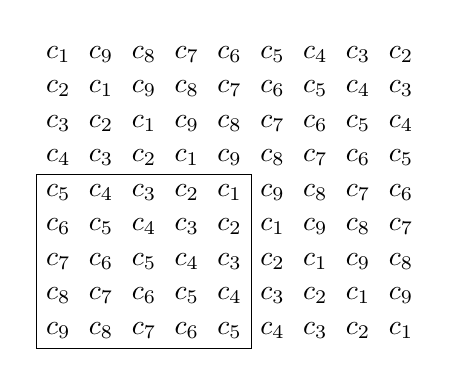
\begin{tikzpicture}
  \matrix (m)[
    matrix of math nodes,
    nodes in empty cells,
    minimum width=width("123"),
  ] {
c_1 & c_9 & c_8 & c_7 & c_6 & c_5 &  c_4 & c_3 & c_2 \\ 
c_2 & c_1 & c_9 & c_8 & c_7 & c_6 &  c_5 & c_4 & c_3 \\ 
c_3 & c_2 & c_1 & c_9 & c_8 & c_7 &  c_6 & c_5 & c_4 \\ 
c_4 & c_3 & c_2 & c_1 & c_9 & c_8 &  c_7 & c_6 & c_5 \\ 
c_5 & c_4 & c_3 & c_2 & c_1 & c_9 &  c_8 & c_7 & c_6 \\ 
c_6 & c_5 & c_4 & c_3 & c_2 & c_1 &  c_9 & c_8 & c_7 \\ 
c_7 & c_6 & c_5 & c_4 & c_3 & c_2 &  c_1 & c_9 & c_8 \\ 
c_8 & c_7 & c_6 & c_5 & c_4 & c_3 &  c_2 & c_1 & c_9 \\ 
c_9 & c_8 & c_7 & c_6 & c_5 & c_4 &  c_3 & c_2 & c_1 \\ 
  } ;
\draw (m-9-1.south west) rectangle (m-5-5.north east);
\end{tikzpicture}
\end{center}
The above circulant matrix is called ${\bf C}_1$. We can create a new vector $\hat{\bf c} = \begin{bmatrix} c_5 & c_6 & c_7 & c_8 & c_9 & c_1 & c_2 & c_3 & c_4 \end{bmatrix}^T$, which is obtained by permutating the elements of the original vector, the Toeplitz matrix can be embedded at the upper-left part of the circulant matrix created from $\hat{\bf c}$ shows as bellow
 \begin{center}
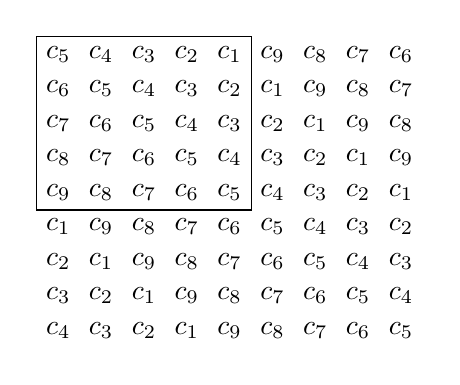
\begin{tikzpicture}
  \matrix (m)[
    matrix of math nodes,
    nodes in empty cells,
    minimum width=width("123"),
  ] {
c_5 & c_4 & c_3 & c_2 & c_1 & c_9 &  c_8 & c_7 & c_6 \\ 
c_6 & c_5 & c_4 & c_3 & c_2 & c_1 &  c_9 & c_8 & c_7 \\ 
c_7 & c_6 & c_5 & c_4 & c_3 & c_2 &  c_1 & c_9 & c_8 \\ 
c_8 & c_7 & c_6 & c_5 & c_4 & c_3 &  c_2 & c_1 & c_9 \\ 
c_9 & c_8 & c_7 & c_6 & c_5 & c_4 &  c_3 & c_2 & c_1 \\ 
c_1 & c_9 & c_8 & c_7 & c_6 & c_5 &  c_4 & c_3 & c_2 \\ 
c_2 & c_1 & c_9 & c_8 & c_7 & c_6 &  c_5 & c_4 & c_3 \\ 
c_3 & c_2 & c_1 & c_9 & c_8 & c_7 &  c_6 & c_5 & c_4 \\ 
c_4 & c_3 & c_2 & c_1 & c_9 & c_8 &  c_7 & c_6 & c_5 \\ 
} ;
\draw (m-5-1.south west) rectangle (m-1-5.north east);
\end{tikzpicture}
\end{center}
 and call this new matrix as ${\bf C}_2$.
 
Suppose we need to compute the product between Toeplitz matrix ${\bf T}$ and a vector ${\bf v}$
\begin{equation}
{\bf r} = {\bf T}{\bf v} \,
\end{equation} 
where the length of ${\bf v}$ is $K$.
There are two way to do it efficiently via FFT, and these two ways corresponding to the two embedding methods. The first step is to padding vector ${\bf v}$ with $L-1$ $0$s get a new vector $\hat{\bf v}$. Following above example, $K=L=5$ and ${\bf v} = \begin{bmatrix} v_1 & v_2 & v_3 & v_4 & v_5  \end{bmatrix}^T$, and the padded vector $\hat{\bf v} = \begin{bmatrix} v_1 & v_2 & v_3 & v_4 & v_5 & 0 & 0 & 0 & 0 \end{bmatrix}^T$, The product between ${\bf C}_1$ and $\hat{\bf v}$ are
\begin{equation}
\hat{\bf r}_1 = {\bf C}_1 \hat{\bf v} = \begin{bmatrix}
c_1 & c_9 & c_8 & c_7 & c_6 & c_5 &  c_4 & c_3 & c_2 \\ 
c_2 & c_1 & c_9 & c_8 & c_7 & c_6 &  c_5 & c_4 & c_3 \\ 
c_3 & c_2 & c_1 & c_9 & c_8 & c_7 &  c_6 & c_5 & c_4 \\ 
c_4 & c_3 & c_2 & c_1 & c_9 & c_8 &  c_7 & c_6 & c_5 \\ 
c_5 & c_4 & c_3 & c_2 & c_1 & c_9 &  c_8 & c_7 & c_6 \\ 
c_6 & c_5 & c_4 & c_3 & c_2 & c_1 &  c_9 & c_8 & c_7 \\ 
c_7 & c_6 & c_5 & c_4 & c_3 & c_2 &  c_1 & c_9 & c_8 \\ 
c_8 & c_7 & c_6 & c_5 & c_4 & c_3 &  c_2 & c_1 & c_9 \\ 
c_9 & c_8 & c_7 & c_6 & c_5 & c_4 &  c_3 & c_2 & c_1 \\ 
\end{bmatrix}
\begin{bmatrix}
v_1 \\
v_2 \\
v_3 \\
v_4 \\
v_5 \\
0 \\
0 \\
0 \\
0 \\
\end{bmatrix}
\end{equation}
where the last $L$ elements of $\hat{\bf r}_1$ equal to ${\bf r}$. On the other hand, we can take advantage of the circulate matrix ${\bf C}_2$, we have
\begin{equation}
\hat{\bf r}_2 = {\bf C}_2 \hat{\bf v} = \begin{bmatrix}
c_5 & c_4 & c_3 & c_2 & c_1 & c_9 &  c_8 & c_7 & c_6 \\ 
c_6 & c_5 & c_4 & c_3 & c_2 & c_1 &  c_9 & c_8 & c_7 \\ 
c_7 & c_6 & c_5 & c_4 & c_3 & c_2 &  c_1 & c_9 & c_8 \\ 
c_8 & c_7 & c_6 & c_5 & c_4 & c_3 &  c_2 & c_1 & c_9 \\ 
c_9 & c_8 & c_7 & c_6 & c_5 & c_4 &  c_3 & c_2 & c_1 \\ 
c_1 & c_9 & c_8 & c_7 & c_6 & c_5 &  c_4 & c_3 & c_2 \\ 
c_2 & c_1 & c_9 & c_8 & c_7 & c_6 &  c_5 & c_4 & c_3 \\ 
c_3 & c_2 & c_1 & c_9 & c_8 & c_7 &  c_6 & c_5 & c_4 \\ 
c_4 & c_3 & c_2 & c_1 & c_9 & c_8 &  c_7 & c_6 & c_5 \\ 
\end{bmatrix}
\begin{bmatrix}
v_1 \\
v_2 \\
v_3 \\
v_4 \\
v_5 \\
0 \\
0 \\
0 \\
0 \\
\end{bmatrix}
\end{equation}
So the first $L$ elements of $\hat{\bf r}_2$ equal to ${\bf r}$. We summarize the efficient computation of the product between Toeplitz matrix and a vector in Algorithm 1 and Algorithm 2
\begin{algorithm}
      \SetAlgoLined
      \Fn{ ${\bf r}= ttv({\bf c}, {\bf v}) $}{
      length of ${\bf c}$: $N = length({\bf c})$   \\
      compute $L = \floor*{\frac{N}{2}}+1$, $K = N+1 - L$   \\
      padding $L-1$ $0$s to the end of ${\bf v}$ to get a new vector $\hat{\bf v}$ with length of $N$\\
      ${\bf r}_1 = {\bf F}_N^{-1} \left(   {\bf F}_N {\bf c} \circ {\bf F}_N  \hat{\bf v}\right) $ \\
      take the last $L$ elements from ${\bf r}_1$ 
      }
      \caption{Teoplitz-Times-Vector}
\end{algorithm}

Another method is summarized in Algorithm 2 as 
\begin{algorithm}
      \SetAlgoLined
      \Fn{ ${\bf r}= ttv({\bf c}, {\bf v}) $}{
      length of ${\bf c}$: $N = length({\bf c})$   \\
      compute $L = \floor*{\frac{N}{2}}+1$, $K = N+1 - L$   \\
      padding $L-1$ $0$s to the end of ${\bf v}$ to get a new vector $\hat{\bf v}$ with length of $N$\\
      move the first $K-1$ element of ${\bf c}$ to the end, get a new vector $\hat{\bf c}$
      ${\bf r}_2 = {\bf F}_N^{-1} \left(   {\bf F}_N \hat{\bf c} \circ {\bf F}_N  \hat{\bf v}\right) $ \\
      take the first $L$ elements from ${\bf r}_2$ 
      }
      \caption{Teoplitz-Times-Vector}
\end{algorithm}

\subsection{Hankel matrix}
We divide Hankel matrices into two classes, one is the number of elements is even and the other one is odd. We first discuss about when the number of elements is even, for example $N=6$. The vector can be expressed as
$${\bf c} = \begin{bmatrix}
c_1\\
c_2\\
c_3\\
c_4\\
c_5\\
c_6\\
\end{bmatrix}$$ 
We follow the $L = \floor*{\frac{N}{2}}+1 = 4$ and $K = N+1-L = 3$ to determine the number of rows and columns of the result Hankel matrix as
\begin{equation}
{\bf H} = 
\begin{bmatrix}
c_1 & c_2 & c_3 \\ 
c_2 & c_3 & c_4 \\ 
c_3 & c_4 & c_5 \\ 
c_4 & c_5 & c_6 \\ 
\end{bmatrix}
\label{eq23}
\end{equation}
We also give the Hermitian transpose (complex-conjugate transpose) of the Hankel matrix as
\begin{equation}
{\bf H}^H = 
\begin{bmatrix}
c_1^*  & c_2^*  & c_3^*  & c_4^*  \\ 
c_2^*  & c_3^*  & c_4^*  & c_5^*  \\ 
c_3^*  & c_4^*  & c_5^*  & c_6^*  \\ 
\end{bmatrix}
\label{eq24}
\end{equation}
where the super-script indicate Hermitian transpose.
We can see that the Hermitian transpose of Hankel matrix is still an Hankel matrix. The vector elements can be determined from the first column and last row. 

\textcolor{red}{Note: The circulant matrix and Teoplitz matrix are constant on the diagonals. However, Hankel matrix are constant on the anti-diagonals.}

One can convert a Hankel matrix to a Toeplitz matrix by reversing its columns. The columns reversing process can be represented by right multiplying a $K \times K$ matrix ${\bf R}$, whose elements are $1$ on the main anti-diagonals and 0 elsewhere. Which given as
\begin{equation}
{\bf T}= \begin{bmatrix}
c_3 & c_2 & c_1 \\ 
c_4 & c_3 & c_2 \\ 
c_5 & c_4 & c_3 \\ 
c_6 & c_5 & c_4 \\ 
\end{bmatrix} = {\bf HR} = 
\begin{bmatrix}
c_1 & c_2 & c_3  \\ 
c_2 & c_3 & c_4  \\ 
c_3 & c_4 & c_5  \\ 
c_4 & c_5 & c_6  \\ 
\end{bmatrix}
\begin{bmatrix}
\quad &  \quad & 1 \\
\quad &  1 & \quad \\
1 &  \quad & \quad \\
\end{bmatrix}
\end{equation}
The columns reverse of the Hermitian transpose of Hankel matrix is also a Toeplitz matrix given as 
\begin{equation}
\hat{\bf T}= \begin{bmatrix}
c_4^* & c_3^* & c_2^* & c_1^* \\ 
c_5^* & c_4^* & c_3^* & c_2^* \\ 
c_6^* & c_5^* & c_4^* & c_3^* \\ 
\end{bmatrix} = {\bf H}^H{\bf R} = 
\begin{bmatrix}
c_1^*  & c_2^*  & c_3^*  & c_4^*  \\ 
c_2^*  & c_3^*  & c_4^*  & c_5^*  \\ 
c_3^*  & c_4^*  & c_5^*  & c_6^*  \\ 
\end{bmatrix}
\begin{bmatrix}
\quad & \quad &  \quad & 1 \\
\quad & \quad &  1 & \quad \\
\quad & 1        &  \quad & \quad \\
1        & \quad &  \quad & \quad \\
\end{bmatrix}
\end{equation}

Before we discuss about the multiplication between Hankel matrix or the Hermitian transpose and a vector, we first look at the property of the column reversing matrix ${\bf R}$, we have 
\begin{equation}
{\bf R} = {\bf R}^T = {\bf R}^{-1}
\end{equation}
So the product between Hankel matrix ${\bf H}$ and a vector ${\bf v}$ is given as 
\begin{equation}
{\bf r} = {\bf Hv} = {\bf HRR}^{-1}{\bf v} = {\bf HRRv} = ({\bf HR})({\bf Rv}) = {\bf T} \hat {\bf v}
\end{equation}
where $\bf{v}$ is the reversed version of the vector ${\bf v}$. Accordingly, the Hermitian transpose of Hankel matrix times a vector can be represented as
\begin{equation}
\hat{\bf r} = {\bf H}^H{v} = {\bf H}^H {\bf RR}^{-1}{\bf v} = {\bf H}^H{\bf RRv} = ({\bf H}^H{\bf R})({\bf Rv}) = \hat{\bf T} \hat {\bf v}
\end{equation}
There are two ways to embed ${\bf HR}$ and ${\bf H}^H {\bf R}$ into a circulant matrix, which is given as
\begin{center}
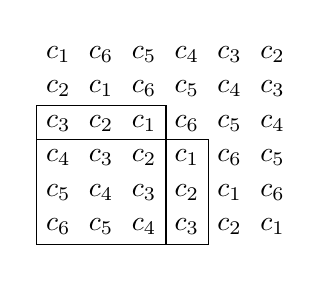
\begin{tikzpicture}
  \matrix (m)[
    matrix of math nodes,
    nodes in empty cells,
    minimum width=width("123"),
  ] {
c_1 & c_6 & c_5 & c_4 & c_3 & c_2 \\ 
c_2 & c_1 & c_6 & c_5 & c_4 & c_3 \\ 
c_3 & c_2 & c_1 & c_6 & c_5 & c_4 \\ 
c_4 & c_3 & c_2 & c_1 & c_6 & c_5 \\ 
c_5 & c_4 & c_3 & c_2 & c_1 & c_6 \\ 
c_6 & c_5 & c_4 & c_3 & c_2 & c_1 \\ 
} ;
\draw (m-6-1.south west) rectangle (m-3-3.north east);
\draw (m-6-1.south west) rectangle (m-4-4.north east);
\end{tikzpicture}
\end{center}
The second way to embed a Hankel matrix into a circulant matrix is given as
\begin{center}
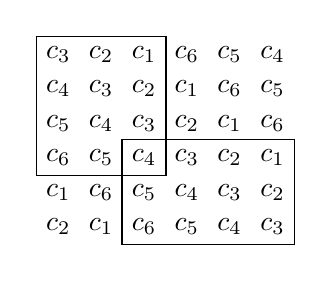
\begin{tikzpicture}
  \matrix (m)[
    matrix of math nodes,
    nodes in empty cells,
    minimum width=width("123"),
  ] {
c_3 & c_2 & c_1 & c_6 & c_5 & c_4 \\ 
c_4 & c_3 & c_2 & c_1 & c_6 & c_5 \\ 
c_5 & c_4 & c_3 & c_2 & c_1 & c_6 \\ 
c_6 & c_5 & c_4 & c_3 & c_2 & c_1 \\ 
c_1 & c_6 & c_5 & c_4 & c_3 & c_2 \\ 
c_2 & c_1 & c_6 & c_5 & c_4 & c_3 \\ 
} ;
\draw (m-4-1.south west) rectangle (m-1-3.north east);
\draw (m-6-3.south west) rectangle (m-4-6.north east);
\end{tikzpicture}
\end{center}

Based on the two different embedding methods, we also have two algorithm to compute the product between Hankel matrix or Hermitian transpose and a vector,  which is given as
\begin{algorithm}
      \SetAlgoLined
      \Fn{ ${\bf r}= htv({\bf c}, {\bf v}; flag="forward" \,\,or\,\,"adjoint") $}{
      length of ${\bf c}$: $N = length({\bf c})$   \\
      compute $L = \floor*{\frac{N}{2}}+1$, $K = N+1 - L$   \\
      reverse the order of the elements of ${\bf v}$: $\hat{\bf v} = reverse({\bf v})$ \\
      Fourier transform: $\hat{\bf c} = fft({\bf c})$ \\
      \If{ Forward}{
      Padding zeros to $\hat{\bf v}$:  $\hat{\bf v} = [\hat{\bf v}, zeros(L-1)]$     \\
      Fourier transform: $\tilde{\bf v}  = fft(\hat{\bf v})$ \\
      element-wise multiplication: ${\bf r} = ifft(\hat{\bf c} \circ \tilde{\bf v})$ \\
      \Return ${\bf r}[K:N]$}
      \If{ Adjoint }{
      Padding zeros to $\hat{\bf v}$:  $\hat{\bf v} = [\hat{\bf v}, zeros(K-1)]$     \\
      Fourier transform: $\tilde{\bf v}  = fft(\hat{\bf v})$ \\
      Conjugate property of Fourier transform: $\tilde{\bf c}[1] = \hat{\bf c}^*[1]$ and  $\tilde{\bf c}[i] = \hat{\bf c}^*[N-i+2] $ \\
      element-wise multiplication: ${\bf r} = ifft(\tilde{\bf c} \circ \tilde{\bf v})$ \\
      \Return ${\bf r}[L:N]$}}
      \caption{Hankel-Times-Vector}
\end{algorithm}
\textcolor{red}{The expression in Line 15 use the conjugate property of Fourier transform, which is stated as}
$$
\mathbfcal{F}[x(t)] \rightarrow X(\omega)$$
$$
\mathbfcal{F}[x^*(t)] \rightarrow X^*(-\omega)
$$

\section{Complex derivative}
Let $f(z, z^{\ast})$: $\mathbb{C} \times \mathbb{C} \rightarrow \mathbb{C}$ be a function of a complex variable $z$ and its complex conjugate $z^{\ast}$, where $z = x + iy$. We have the derivative 
\begin{equation}
\frac{\partial f}{\partial z} = \frac{1}{2}(\frac{\partial f}{\partial x} - i\frac{\partial f}{\partial x}),
\end{equation}
and
\begin{equation}
\frac{\partial f}{\partial z^{\ast}} = \frac{1}{2}(\frac{\partial f}{\partial x} + i\frac{\partial f}{\partial x}).
\end{equation}
Using the definition of complex derivative, it's clear that 
\begin{equation}
\begin{split}
\frac{\partial f}{\partial z} &= \left( \frac{\partial f}{\partial z^{\ast}} \right)^{\ast} \\
\frac{\partial z}{\partial z} &= 1 \\
\frac{\partial z^{\ast}}{\partial z^{\ast}} &= 1 \\
\frac{\partial z^{\ast}}{\partial z} &= 0
\end{split}.
\end{equation}
With above property, we can simply consider the complex variable and its complex conjugate $z^{\ast}$ as two independent variable. 

\subsection{Stationary point}
Let $f(z, z^{\ast})$: $\mathbb{C} \times \mathbb{C} \rightarrow \mathbb{R}$ be a function mapping a complex variable $z$ and its complex conjugate $z^{\ast}$ to a real number. A sufficient and necessary condition for $f(z, z^{\ast})$ have a stationary point is $\frac{\partial f}{\partial z} = 0$. Similarly $\frac{\partial f}{\partial z^{\ast}} = 0$ is also a sufficient and necessary condition.

\subsection{Complex gradient}
Let's think about the first-order Taylor-series expansion, we have 
\begin{equation}
\delta f = \frac{\partial f}{\partial z} \delta z +  \frac{\partial f}{\partial z^{\ast}} \delta z^{\ast} 
\end{equation}
By using the property $\frac{\partial f}{\partial z} = \left( \frac{\partial f}{\partial z^{\ast}} \right)^{\ast}$, we can get 
\begin{equation}
\delta f = 2 Re (\frac{\partial f}{\partial z} \delta z),
\end{equation}
where the operator $Re$ means take the real part of the input.
We can extend this property to a function of a complex vector $g$: $\mathbb{C}^N \rightarrow \mathbb{R}$. We denote the complex vector as $\bf z$, so its first-order Taylor expansion can be expressed as
\begin{equation}
\begin{split}
\delta g &= 2 \sum_{i=1}^N Re \left(\frac{\partial g}{\partial z_i} \delta z_i \right) \\
             &= 2 Re\left( \left( \frac{\partial g}{\partial {\bf z}} \right)^T {\bf \delta z} \right)
\end{split}
\end{equation}
To make the above expression consistent with the axiom of inner product, we replace the above equation as 
\begin{equation}
\delta g = 2 Re \left( \left( \frac{\partial g}{\partial {\bf z^{\ast}}}\right)^H {\bf \delta z} \right)
\end{equation}
The maximum change $\delta g$ is obtained when $\delta {\bf z}$ is in the same direction of $\frac{\partial g}{\partial {\bf z^{\ast}}}$. It means that
\begin{equation}
\delta {\bf z} = \alpha \frac{\partial g}{\partial {\bf z^{\ast}}}.
\end{equation}
Where $\alpha$ is a real number indicate the magnitude of the vector $\delta {\bf z}$. This explanation suggest that the gradient vector $ \frac{\partial g}{\partial {\bf z^{\ast}}}$ is required for updating the variable ${\bf z}$ in an optimization problem.

\subsection{discrete time linear time invariant system}
We derive the mathematical model for describing discrete time linear invariant system. Suppose the input to a system is an impulse $\delta[n]$, which is equal to $1$ when $n=0$ and is $0$ elsewhere. The impulse response of this system is indicated by $h[n]$. The $\textbf{time invariant}$ property mean that the delayed impulse response is the output of the delayed impulse, which can be expressed as 
\begin{equation}
\delta[n-k] \rightarrow h[n-k],
\end{equation}
where $k$ indicate the number of samples delayed.

Any discrete-time signal(sequence) can be expressed as the weighted summation of delayed impulse as 
\begin{equation}
x[n] = \sum_{k=-\infty}^{+\infty} x[k] \delta[n-k]
\label{input}
\end{equation}
Combine with the linear property of this system, the output can be expressed as
\begin{equation}
y[n] = \sum_{k=-\infty}^{+\infty} x[k] h[n-k]
\end{equation}
Which give the definition of convolution which are used to describe the linear time-invariant system as $y[n] = x[n] \ast h[n]$.

Suppose the input is given as $g[n] = x[n-p_1]$ and the impulse response of the system is $f[n] = h[n-p_2]$. What is the output of this system? There are two ways to derive the result, one is based on the definition we given in equation (\ref{input}).
\begin{equation}
\begin{split}
g[n] &= \sum_{k=-\infty}^{+\infty} g[k] \delta[n-k] \\
       &= \sum_{k=-\infty}^{+\infty} x[k-p_1] \delta[n-k]
\end{split}
\end{equation}
The output of this system is
\begin{equation}
\begin{split}
s[n] &= \sum_{k=-\infty}^{+\infty} x[k-p_1] f[n-k] \\
       &= \sum_{k=-\infty}^{+\infty} x[k-p_1] h[n-k-p_2] \\
\end{split}
\label{sum}
\end{equation}
We can the variable change trick by setting $k^{\prime} = k-p_1$, so we have $k = k^{\prime} + p_1$. With this variable change, equation (\ref{sum}) can be reformulated as 
\begin{equation}
\begin{split}
s[n]  &= \sum_{k^{\prime}=-\infty}^{+\infty} x[k^{\prime}] h[n-k^{\prime}-p_1- p_2]    \\
        &= \sum_{k^{\prime}=-\infty}^{+\infty} x[k^{\prime}] h[(n-p_1- p_2)-k^{\prime}] \\
        &= y[n-p_1-p_2]
\end{split}
\label{sum}
\end{equation}


\bibliographystyle{seg}
\bibliography{paper}

\end{document}

